\subsection{Metriche software}

\subsubsection{Versioni del browser supportate}
\begin{figure}[h]
	\centering
	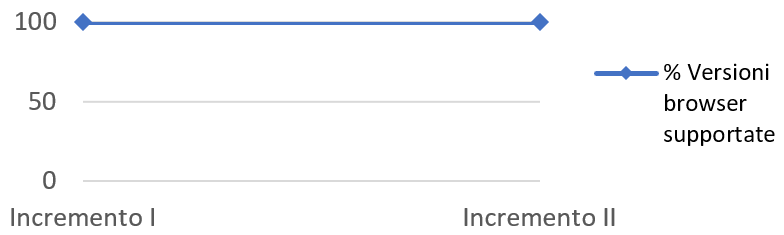
\includegraphics[width=11cm]{Images/vBrowser}
	\caption{Grafico delle versioni browser supportate.}
\end{figure}

\subsubsection{Facilità di utilizzo}
\begin{figure}[h]
	\centering
	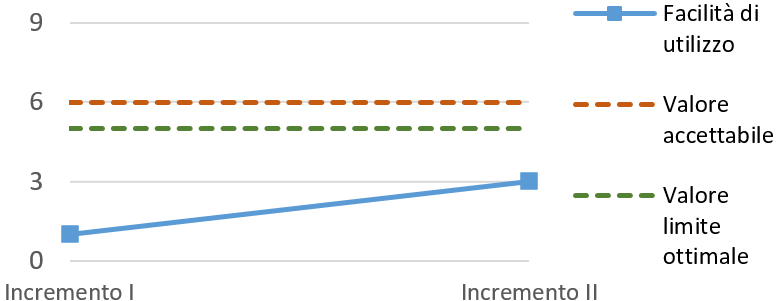
\includegraphics[width=11cm]{Images/facUtilizzo}
	\caption{Grafico della facilità di utilizzo.}
\end{figure}

\subsubsection{Copertura dei requisiti}
\begin{figure}[h]
	\centering
	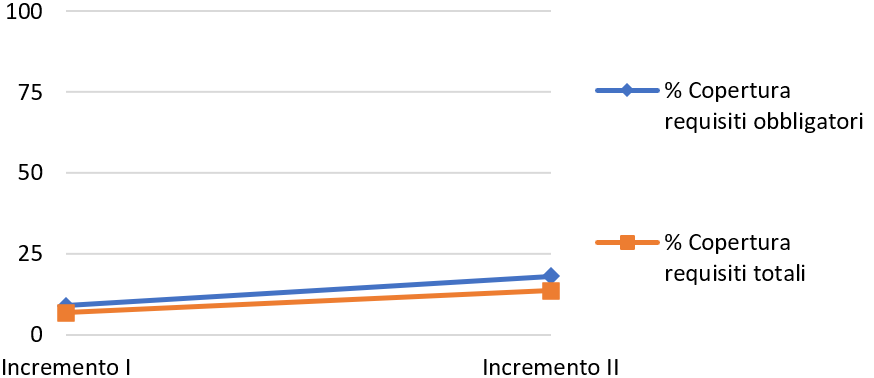
\includegraphics[width=11cm]{Images/copRequisiti}
	\caption{Grafico del numero di requisiti soddisfatti.}
\end{figure}

\subsubsection{Average Cyclomatic complexity}
\begin{figure}[h]
	\centering
	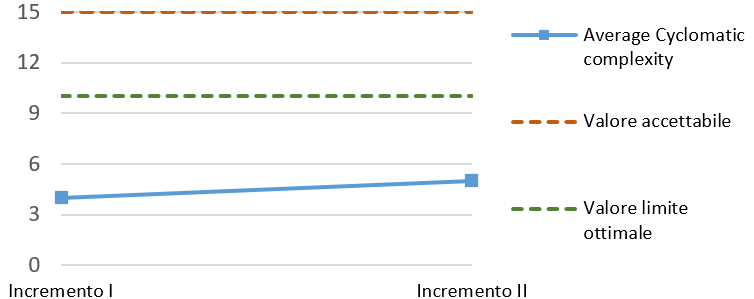
\includegraphics[width=14cm]{Images/avComplex}
	\caption{Grafico complessità ciclomatica.}
\end{figure}

\subsubsection{Tempo medio di risposta}
\begin{figure}[h]
	\centering
	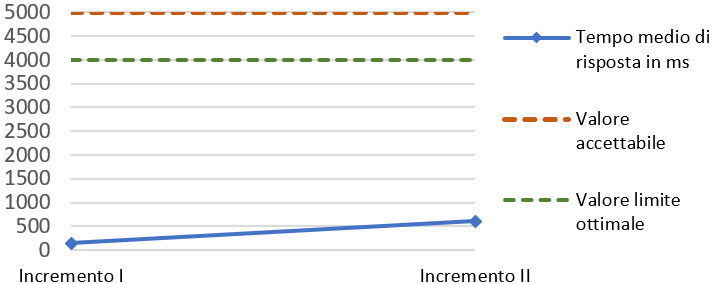
\includegraphics[width=14cm]{Images/tRisp}
	\caption{Grafico risposta media.}
\end{figure}

\newpage

\subsubsection{Facilità apprendimento funzionalità}
\begin{figure}[h]
	\centering
	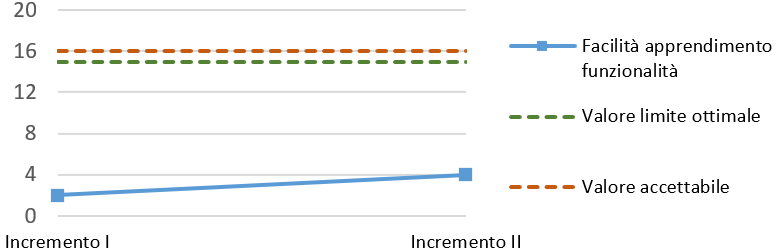
\includegraphics[width=14cm]{Images/fAppr}
	\caption{Grafico della facilità di apprendimento.}
\end{figure}